\section{Module 2: Lecture 1\\Sinusoidal Signals and their Properties}

\subsection*{Introduction}
In the first module, we have been looking at signals and systems in what is
called their natural domain. By natural domain, we mean that the independent
variable of the signal is the same as it was when the signal was
recorded or observed or instituted. An example of a signal in its natural
domain is a speech signal expressed as a function of time, as time is the
naturally associated independent variable with the speech signal. \\
For processing signals, we need appropriate systems. Now, what processing needs to be done by the system can be a tricky thing to specify in the
natural domain. \\
For example, say we want to separate the voices of male and female
singers from an audio recording of a chorus. Although it is qualitatively easier to understand, one can't give the description of such a system in the
time domain. We need to
have a broader view of systems, and more importantly, of signals, to be able
to tackle this problem. \\
So in this module we are going to take the first step towards a change of
paradigm, a change of world-view in describing signals and systems.
%% Adding the Introduction from M2L02 here as of now.
In this lecture we will learn how to deal with phase changes in sinusoidal signals and pass sinusoidal signals into stable LSI systems in an intelligent and insightful manner. We will look into why we introduced complex signals in our previous analysis and how these tools make the mathematical modelling simple. We then go on to understanding how to deal with signals beyond the domain of sinusoids.
%% Intro of M2L02 ends here
We begin by understanding which signals are special from the point of view of
the signals and systems. Let's visit the ideal voltage generator for that
purpose.
\subsection{The Ideal Voltage generator}
The ideal voltage generator consists of a circular conducting coil rotating in
a constant magnetic field.
\begin{figure}[ht]
\centering
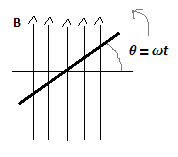
\includegraphics{flux.png}
\caption{\label VVoltage generator (side view)}
\end{figure}
\\
Let the area enclosed by the coil be $A$, the angular frequency of
rotation be $\omega$ such that $\theta = \omega t$, and the value of the
constant magnetic field be $B$. Now, by Faraday's law, the electric field $\mathcal{E}$ is defined as
\[ \mathcal{E}= - \frac{\partial \Phi_B}{\partial t} \]
where the flux $\Phi_B$ in this case is given by
\[ \Phi_B = BA \cos \theta = BA \cos \omega t \]
Hence the electric field will be
\[ \mathcal{E}= - BA \ \omega \sin \omega t \]
This is the principle of generation of the voltage supply that we receive at
our residences. This is one important reason why the sinusoidal voltage is
highly favoured and deeply studied. And of course there are many other reasons
why. Let us have a look at some interesting properties of sinusoids.
%%%
%%%
\subsection{Properties of sinusoids}
The first interesting thing about sine waves is that when you add two sinusoids
of the same frequency, it gives you back another sinusoid of the \emph{same}
frequency. Let's prove this formally.
Say we have two sinusoids, $x_1 (t)$ and $x_2 (t)$, of the same angular frequency
$\Omega,$ given by
\begin{equation*}
x_1 (t) = A_1 \cos (\Omega t + \phi_1)
\end{equation*}
\begin{equation*}
x_2 (t) = A_2 \cos (\Omega t + \phi_2)
\end{equation*}
Now consider a linear combination of the two sinusoids,
\begin{equation*}
x (t) = \alpha_1 x_1 (t) + \alpha_2 x_2 (t)
\end{equation*}
Note that we can write $x_1$ and $x_2$ as
\begin{equation*}
x_1 (t) = A_1  \{ \cos \Omega t \cos \phi_1 - \sin \Omega t \sin \phi_1 \}
\end{equation*}
\begin{equation*}
x_2 (t) = A_2  \{ \cos \Omega t \cos \phi_2 - \sin \Omega t \sin \phi_2 \}
\end{equation*}
Hence we can write $x (t)$ as
\begin{equation*}
x (t) = [ \alpha_1 A_1 \cos \phi_1 + \alpha_2 A_2 \cos \phi_2 ] \cos
   \Omega t + [ - \alpha_1 A_1 \sin \phi_1 - \alpha_2 A_2 \sin
   \phi_2 ] \sin \Omega t
\end{equation*}
Writing the two time-independent coefficients as $P$ and $Q$, we get
\begin{equation*}
 x (t) = P \cos \Omega t + Q \sin \Omega t = \sqrt{P^2 + Q^2}  \left\{
   \frac{P}{\sqrt{P^2 + Q^2}} \cos \Omega t + \frac{Q}{\sqrt{P^2 + Q^2}}
   \sin \Omega t \right\}
\end{equation*}
This can be easily seen to be
\begin{equation*}
 x (t) = \sqrt{P^2 + Q^2} \cos (\Omega t + \Phi)
\end{equation*}
with
\begin{equation*}
\Phi = - \tan^{- 1} \left( \frac{Q}{P} \right)
\end{equation*}
Hence, linearly combining two sinusoids of the same frequency gives back a
sinusoid with the same frequency.\\
Another interesting property is that when we differentiate a
sine wave, we get back a sinusoid of the same frequency.
\begin{equation*}
\frac{d}{d t}  \{ A \cos (\Omega t + \phi) \} = - A \Omega \sin
   (\Omega t + \phi)
\end{equation*}
It doesn't matter whether it is cosine or sine since they differ only by a
phase of $\pi / 2$.
\[ \cos (\Omega t + \phi) = \sin (\Omega t + \phi + \pi / 2) \]
Now let's see how we can describe a change in amplitude of a sinusoid.
Suppose the original sinusoid is given by
\[ x_1 (t) = A \cos (\Omega t + \phi) \]
and let the changed sinusoid is given by
\[ x_2 (t) = B \cos (\Omega t + \phi) \]
where $A$ and $B$ are positive constants. Then,
\[ x_2 (t) = \frac{B}{A} x_1 (t) \]
So the change of amplitude in a sinusoid is simply described by a multiplying
constant.\\
But this is not true for a phase change. Suppose the original sinusoid is
given by
\[ x_1 (t) = A \cos (\Omega t + \phi_1) \]
and the changed sinusoid is given by
\[ x_2 (t) = A \cos (\Omega t + \phi_2) \]
Unlike the amplitude case, $x_2 (t) / x_1 (t)$ doesn't turn out to be a
constant independent of time. This will cause a problem while dealing with
inductors or capacitors. In inductors, for example, the voltage drop is
proportional to the derivative of the current passing through it. Hence, if a
sinusoidal current is passing through it, the voltage drop across it will also
be a sinusoid, but will have a phase difference of $90^0$ with the current.
Hence, we cannot establish a relationship like the resistor $(V = RI)$ in case
of the inductor since $V / I$ won't be a constant independent of time.\\
To deal with this problem, we will have to use the rotating complex number
representation of the sinusoid.

\subsection{Sinusoids as Rotating Complex Numbers}

We can think of a sinusoid $I_0 \cos (\Omega t + \phi_0)$ as a combination of
two rotating complex numbers. Let the first begin at time $t = 0$ with an
angle of $\phi_0$. Let it have a magnitude of $I_0 / 2$ and let the other
begin with the same magnitude $I_0 / 2$ but the opposite starting angle ($-
\phi_0$). Let them both rotate with an angular velocity of $\Omega$, but the
first one in counter clockwise and the second one in clockwise direction.
\begin{figure}[ht]
\centering
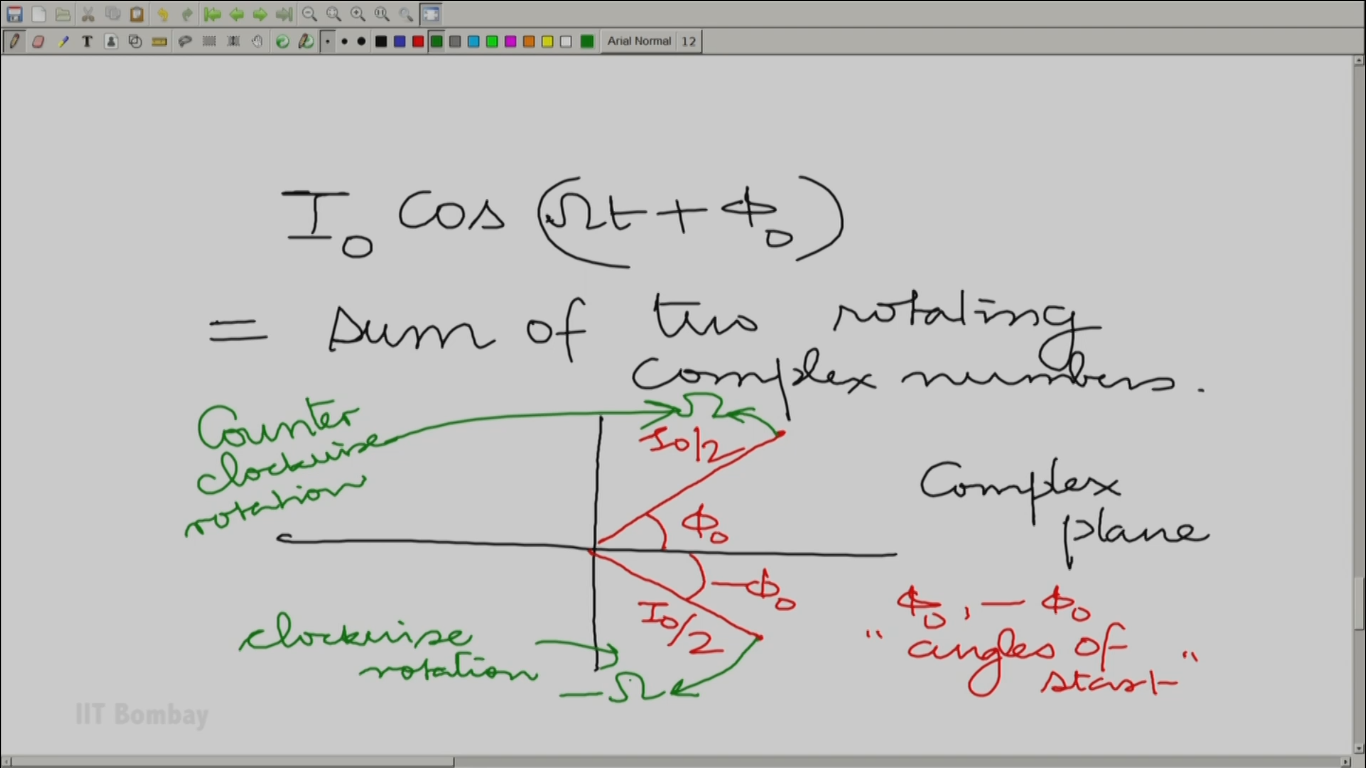
\includegraphics[scale=0.28]{rotating_complex.png}
\end{figure}
\\
We can express these two complex numbers in the polar form as
\[ c_1 = \frac{I_0}{2} e^{j \{ \Omega t + \phi_0 \}} \]
\[ c_2 = \frac{I_0}{2} e^{- j \{ \Omega t + \phi_0 \}} \]
where $j = \sqrt{- 1}$. One can see that $c_1 + c_2$ gives back the original
sinusoid.\\
It seems like a silly thing to do to describe a sinusoid as a combination of
two rotating complex numbers. But the reason for doing this is clear when we
look at the inductor once again.\\
Let's assume for now that we provide to the inductor, an input which is just
one of those rotating complex numbers. So
\[ I = \frac{I_0}{2} e^{j \{ \Omega t + \phi_0 \}} \]
Now, the voltage across an inductor is given by
\[ V = L \frac{d I}{d t} = L\frac{I_0}{2} (j \Omega) e^{j \{ \Omega t +
   \phi_0 \}} \]
Hence we can see that
\[ V / I = j \Omega L \]
Now the ratio of the voltage and current for an inductor is a complex
\textit{constant independent of time}!\\
Similarly, for the other rotating complex number, we will get $V / I$ again to
be a constant, but with a minus sign $(- j \Omega L)$. So in some sense the
actual angular frequency, whether positive or negative, is reflected. It is left as an exercise to do a similar analysis for capacitances and verify that
for capacitors,
\[ V / I = \frac{1}{j \Omega C} \]
This makes the analysis of RLC circuits (circuits consisting of Resistor(s),
Inductor(s) and Capacitors(s)) much easier as we can interpret these constants
as generalised resistances, or \textit{impedances.} In that sense, the
resistor has an impedance of $R$, an inductor has an inductance of $j \Omega
L$ and a capacitor has an impedance of $1 / j \Omega C$.\\
Notice that $c_1$ and $c_2$ defined above are complex conjugates of each
other. So whatever happens to $c_1$ is mirrored in $c_2$. For example, the $V
/ I$ for $c_2$ ($- j \Omega L$) is the complex conjugate of the $V / I$ for
$c_1$ ($j \Omega L$).\\
The analysis of sinusoids using rotating complex numbers is known as `phasor'
analysis. As the rotating complex numbers are constant in magnitude, but
change their phase, they are called `phasors'.\\
This is the reason why we earlier demanded that our systems should accept a
complex signal in general.\\
In a nutshell, dealing with amplitudes is easy but the dealing with phases is
a problem in sinusoids and that problem is overcame when you go to the phasor
instead of the corresponding sinusoid. Let us see how a general LSI system responds to
a phasor or sinusoid as an input.